% !TEX root = ../CedricDe Schepper2023_Thesis.tex

\section{Method}\label{sec:method}
For this thesis, the \acrlong{tabu} algorithm, as proposed by Alvarez-Valdes et al. \cite{alvarez1997}, is used to conduct our experiments. \acrshort{tabu} was chosen for several reasons. First, the simple nature of \acrshort{tabu} improves the interpretability and explainability of the method. The interpretability is important when trying to improve an algorithm based on its results. Only after understanding why a search method behaves a certain way can it efficiently be improved. High explainability makes it easier to explain the used algorithm to university administrators. Secondly, the tabu list prevents cycling between a set of states, which can reduce the amount of time needed to converge. Finally, it has been shown that \acrlong{tabu} is able to outperform other competitive algorithms  on data sets specific to institutions \cite{alvarez1997} \cite{colorni1999} \cite{Chu2000} as well as standardised benchmarks \cite{gaspero2001}.  

\subsection{Tabu Search}

 \acrfull{tabu}\cite{glover1993} starts by constructing an initial solution. The solution can be generated randomly or by applying a deterministic approach. During the entire process, both the best seen solution to date and the current solution are maintained. Keeping the best seen solution is necessary in order to allow the current solution to accept allowing worsening changes. This helps \acrshort{tabu} to avoid getting trapped in local minima. After the solution initialisation, the iterative procedure starts searching for a feasible solution. This loop ends when  a specified stopping condition is met. This condition is generally a combination of a solution its objective function scoring below a certain threshold or the procedure reaching a maximum number of iterations.
\\\\
The first step of the main loop generates the complete list of possible neighbours for the current solution and ranks them based on the objective function. Subsequently, the best neighbour, for which the required move is either not tabu or that meets the aspiration criterion, is chosen as the next solution. A move is considered tabu if it is present within the tabu list, meaning it has been used recently. The aspiration criterion is added to be able to override the tabu requirement. A possible aspiration is to accept solutions that are better than the best seen solution. After choosing the next solution, the best seen solution is updated if the newly generated solution is superior based on the objective function.
\\\\
When the stopping criteria is met, the algorithm ends and the best solution is returned. The full flow of the algorithm can be seen in figure \ref{fig:tabu-chart}.

\begin{figure}[h]
	\centering
	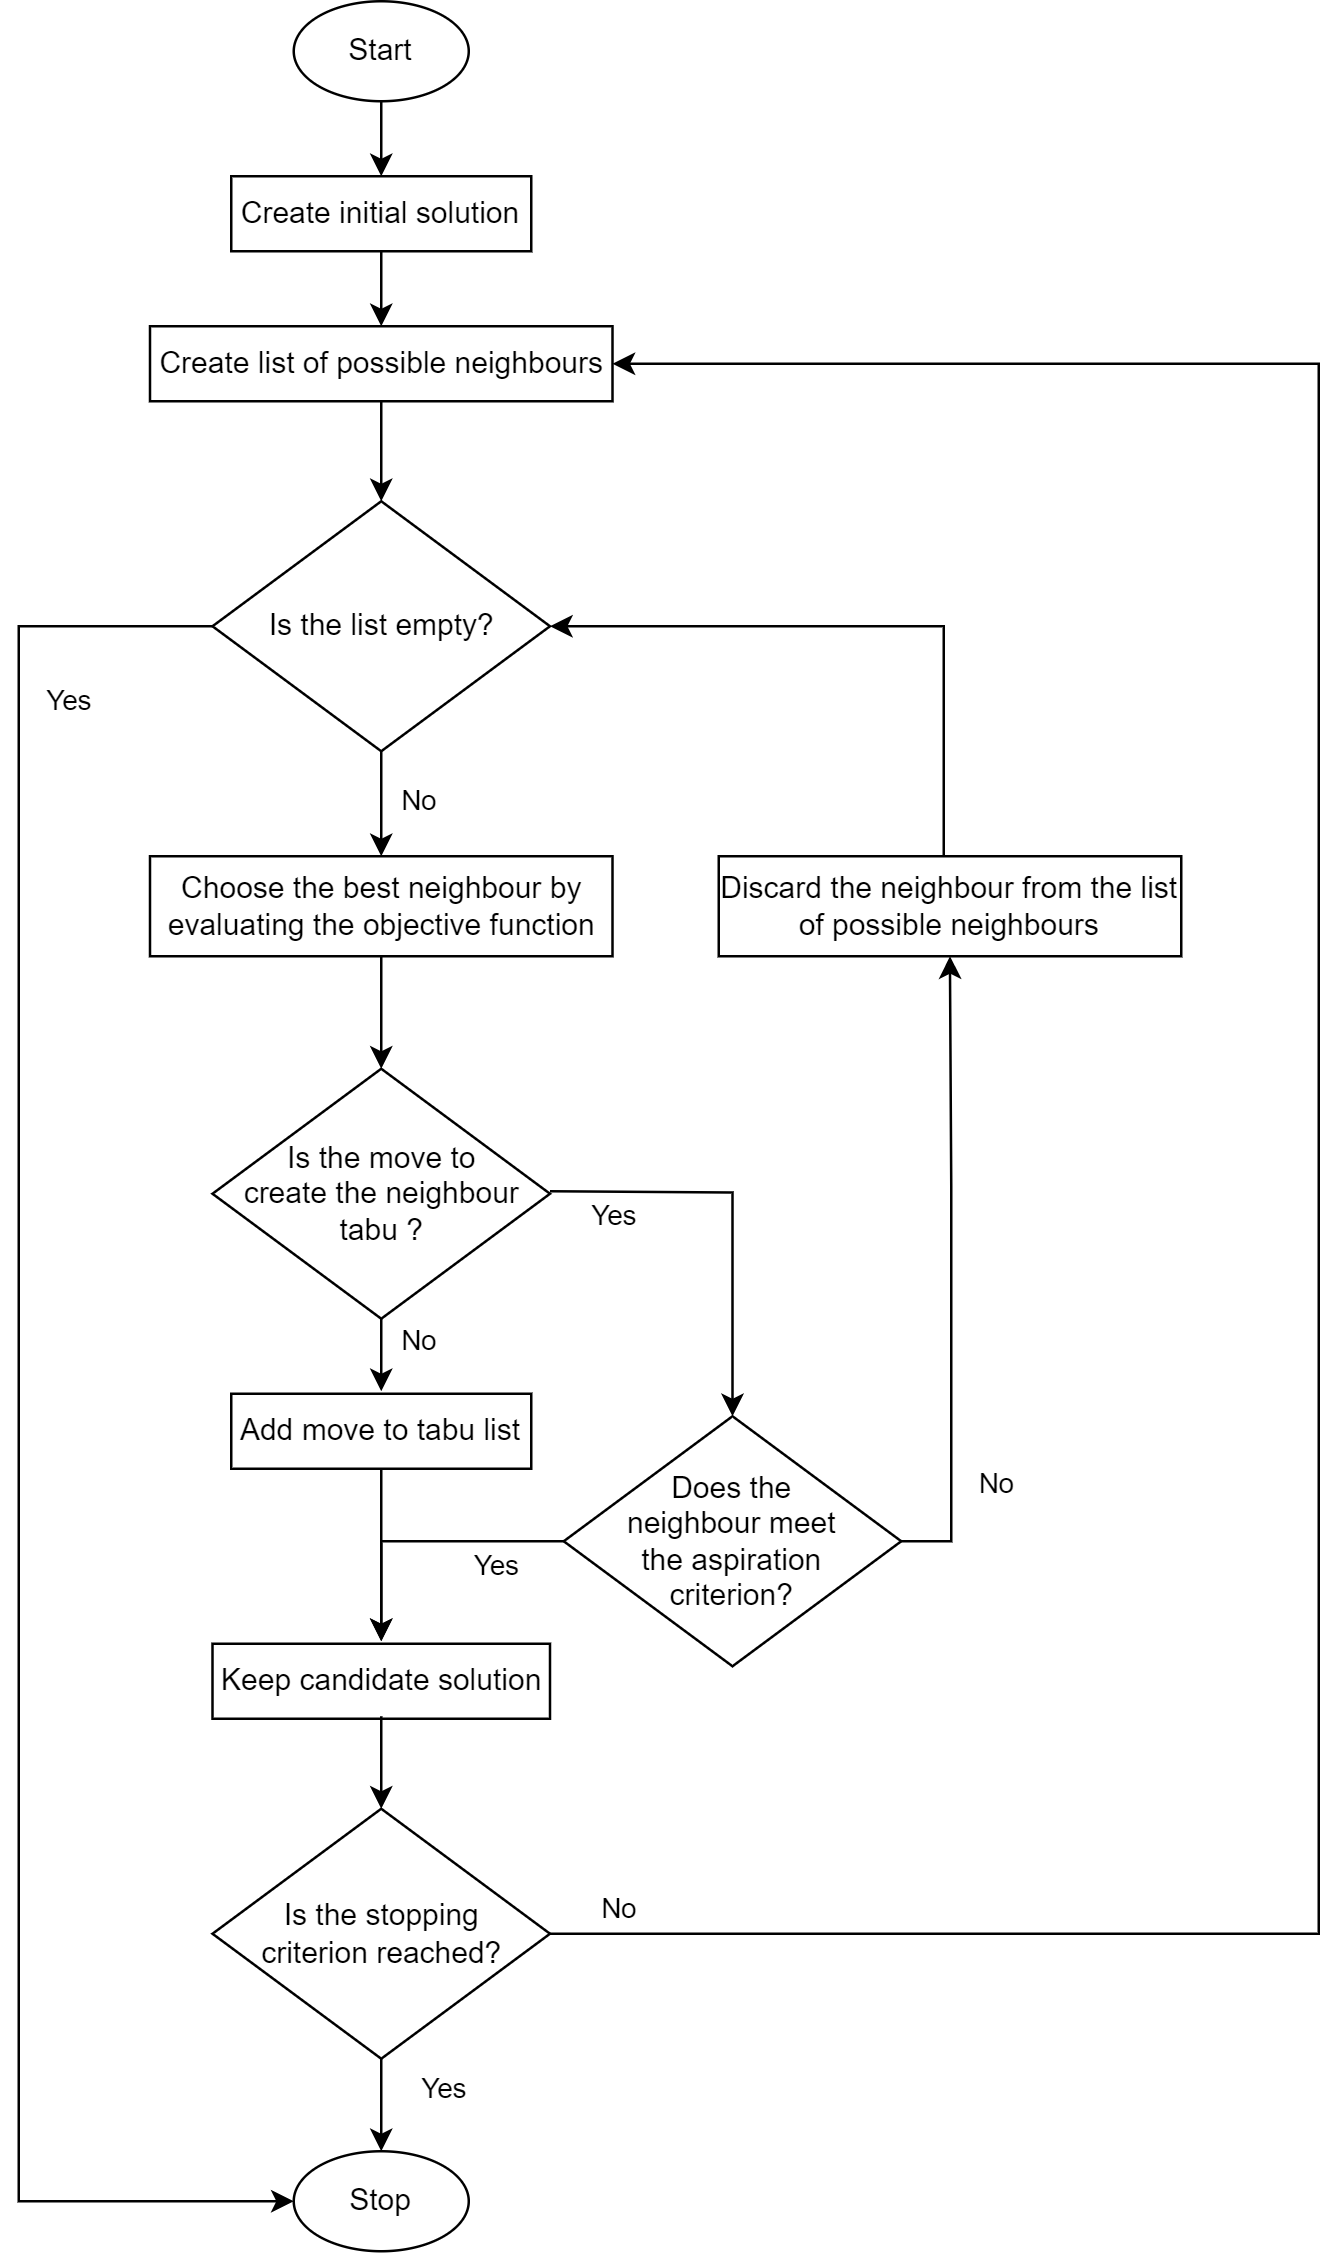
\includegraphics[width=0.8\textwidth]{images/tabu.png} 
	\caption{\acrlong{tabu} flow}
	\label{fig:tabu-chart}
\end{figure}

\subsection{Implementation frameworks}

The algorithm implemented to run the experiments is written using Python3.10. The code requires no packages that are not in the Python Standard Library. The profiler cProfiler is used to analyse the performance. It generates a list detailing how long each part of the algorithm runs for and allows to pinpoint and improve bottlenecks.

\subsection{Version 1: base algorithm}
The proposed algorithm makes use of a 2-phased approach. During phase 1, the emphasis is on the hard constraints. More specifically, reducing the amount of common students conflicts on the same day is prioritised. Optimally, this initialisation phase would return a solution that is already feasible. The second phase can be considered an optimisation phase, which tries to satisfy the soft constraints as much as possible and thus attempt to distribute the exams evenly.

\subsubsection{Initialisation phase}
The algorithm starts with the initialisation for which the pseudo code is shown in Algorithm \ref{alg:phase1}. First, the initial solution must be generated. In the proposed algorithm this is done by randomly assigning all exams to time slots. Generally, this will result in several hard constraint violations, such as students having more than 1 exam on the same day and room capacity being exceeded. Since Alvarez-Valdes et al. consider the room capacity a soft constraint, this is acceptable and will be improved during the iterations. However, in this case, room capacity is seen as a hard constraint that can't be violated at all. In order to circumvent these capacity violations, exams are sorted by student count and only then randomly assigned to time slots with rooms having sufficient capacity. As long as the time slot quantity and room capacity is sufficient, this will result in a solution with no room capacity violations. Another added complexity is the presence of different room types which was not the case for Alvarez-Valdes et al. In order to satisfy constraint 2, only rooms with a suitable type are considered when assigning exams to time slots.

\begin{algorithm}
 Generate an initial solution s in the space of solutions X\;
 $s^* = s$ (with $s^*$ the best solution seen so far)\;
 $k = 0$ (with k the number of iterations)\;
 \While{k < maximum number of iterations and $f(s^*) \neq 0$}{
  $k = k + 1$\;
  \tcc{perform single moves of one exam to another time slot}
  Generate set of solutions $V^* \subseteq N(s, k)$\ (set of neighbours of s)\;
  Sort $V^*$ by ascending $f(s')$ and select the best $s'$\;
   \ForEach{solution $s'$ in $V^*$}{
    \If{not $tabu(s')$ or $f(s') < f(s^*)$ (aspiration criterion)}{
        $s = s'$\;
        \textbf{break}\;
    }
   }
   \If{$f(s') < f(s^*)$}{
   $s^* = s'$\;
   }
 }
 \KwRet{$s^*$}

\caption{Initialisation phase}
\label{alg:phase1}
\end{algorithm}

After generating the initial solution, the iterative procedure starts by generating the set of neighbours of the current solutions. In the search space $X$, we consider a solution $s' \in X$ a neighbour of $s \in X$, whenever we can move an exam to a time slot in a different period. Evaluating the entire search space would be too time consuming. Instead, we first sort all periods by its contribution to the objective function. From the most conflictive period, we select the most conflictive time slot. Finally, we calculate all available time slots that we can swap with. In order to swap two time slots, the two affected exams (or sole affected exam when swapping to a time slot with no scheduled exam) must be able to be scheduled in the new time slots keeping the room type and capacity into account. This will ensure that no additional constraint 2 and 3 violations are introduced.

For each possible move, the objective score is calculated in order to rank all neighbours. The objective function for a solution $s$ is defined as

\begin{equation}
    f(s) = \sum_{i=1}^{P} \left( \sum_{j \in E_i}^{}\sum_{k \in E_i \atop k \neq j}^{}w \lvert S_j \cap S_k \rvert \right)
\end{equation}


with $P$ the amount of periods, $E_i$ the set of exams scheduled to period $i$, $S_j$ and $S_k$ the students scheduled to exam $j$ and exam $k$ respectively. This makes $\lvert S_j \cap S_k \rvert$ the amount of common students between the two exams. Lastly, the weight of student conflicts is denoted by $w$.

After sorting all found neighbours by objective function, the best solution, that is not tabu or for which the aspiration criterion applies, is chosen. The aspiration criterion accept a solution, for which the required move is tabu, as long as it is superior to $s^*$ (the best solution seen so far). If no moves are possible, we select the next most conflictive time slot until a suitable move has been found. When choosing the new solution, the tabu list is updated with the new tabu move consisting of the exam and period involved. Whenever the tabu list exceeds its maximum size, the oldest move is deleted, in order to allow that move again in future iterations.

Alvarez-Valdes et al. calculate the size of the tabu list as

\begin{equation} \label{eq:list}
    \text{Tabu list size} = \lfloor\sqrt{\text{\# Exams} * \text{\# Periods}}\rfloor
\end{equation}

This initialisation phase runs until a solution without conflicts has been found or the maximum number of iterations has been reached. For the latter case, the schedule will have conflicting exams during the same period with common students.

\subsubsection{Optimisation phase}

After the initialisation phase, we start the optimisation of the solution. Here the focus is including the soft constraints in the objective function to generate a solution that is the most optimal. The foundation of this phase is similar compared to the first phase with some distinct features. The overall flow can be seen in the pseudo code described in Algorithm \ref{alg:phase2}.

\begin{algorithm}
\KwData{Solution s (the result of the initialisation phase)}
 $s^* = s$ (with $s^*$ the best solution seen so far)\;
 $k = 0$ (with k the number of iterations)\;
 \While{k < maximum number of iterations and $f(s^*) \neq 0$}{
  $k = k + 1$\;
  \uIf{$k\ \mathbf{mod}\ 3 \neq 0$}{
  \tcc{perform single moves of one exam to another time slot}
    Generate set of solutions $V^* \subseteq N(s, k)$\ (set of neighbours of s after single move)\;
  Sort $V^*$ by ascending $f(s')$ and select the best $s'$\;
   \ForEach{solution $s'$ in $V^*$}{
    \If{not $tabu(s')$ or $f(s') < f(s^*)$ (aspiration criterion)}{
        $s = s'$\;
        \textbf{break}\;
    }
   }
  }
  \Else{
    \tcc{swap entire period}
    Generate set of solutions $V^* \subseteq N(s, k)$\ (set of neighbours of s after swapping periods)\;
    Sort $V^*$ by ascending $f(s')$ and select the best $s'$\;
    $s = s'$\;
  }
  
   \If{$f(s') < f(s^*)$}{
   $s^* = s'$\;
   }
 }
 \KwRet{$s^*$}

\caption{Optimisation phase}
\label{alg:phase2}
\end{algorithm}


First, the objective function is updated to take the distribution of exams into account. The objective of a solution is now defined as

\begin{equation}
    f(s) = \sum_{i=1}^{P} \sum_{j=i}^{P}\left(w_{|i-j|} \sum_{k \in E_i}^{}\sum_{l \in E_j \atop k \neq l}^{} \lvert S_k \cap S_l \rvert\right)
\end{equation}
with $P$ the amount of periods, $E_i$ the set of exams scheduled to period $i$, $S_k$ and $S_l$ the students scheduled to exam $k$ and exam $l$ respectively. This makes $\lvert S_k \cap S_l \rvert$ the amount of common students between the two exams. Here, the weight $w$ is dependent on the amount of days between the exams, with $w_i$ the weight for exams scheduled $i$ days apart.

While the objective function in the first phase only used the common students between exams during the same period, the new objective function will take all periods into account. Constraint 5a, that does not allow students having more than one exam on the same day, is now relaxed to constraint 5b. By having a large weight $w_0$ for two exams scheduled on the same day, these exam conflicts for non-model track are only introduced if the decrease of the objective function is significant. Additionally, placing exams at a further distance will now be preferred since the weight $w_{x+1}$ will be smaller than the weight $w_x$.


Secondly, two options are now available when generating the set of neighbours of the solution. The first option is a copy of the process in the initialisation phase where the set of neighbours of the solution is generated by performing single moves. Then the best solution that is either not tabu or that meets the aspiration criterion will be used. While this option might introduce constraint violations, the high $w_0$ will discourage and, depending on the values used, prevent this. This method will be alternated with a period permutation. Instead of moving a single exam, two entire periods will be swapped. Since the exams in the periods are not updated, this swap can not introduce any hard constraint violations. By moving entire periods, the objective function can change significantly in a single move. However, the amount of available moves is much lower and can be defined as
\begin{equation}
\begin{split}
   \text{\# possible moves}  & = \binom{P}{2}   \\
   & = \frac{P!}{2!(P-2)!}
\end{split}
\end{equation}

\subsection{Version 2: updating the objective function and tabu move definition}

We propose an altered version that builds on the base algorithm by changing two key aspects. First, we noticed that the objective function originally defined in the initialisation phase as   
\begin{equation}
    f(s) = \sum_{i=1}^{P} \left( \sum_{j \in E_i}^{}\sum_{k \in E_i \atop k \neq j}^{}w \lvert S_j \cap S_k \rvert \right)
\end{equation}

has an unwanted characteristic for our case: it does not punish students with several exams on the same day extra. For exam schedules without a conflict free solution, this often results in students, who are enrolled in smaller exams, having a large number of exams on the same day. In order to avoid this behaviour, the objective function is updated to
\begin{equation}
    f(s) = \sum_{i=1}^{P} \left( \sum_{s \in S(E_i)}^{}w^{c_{s,i} - 1}\right)
\end{equation}
with $P$ the amount of periods, $E_i$ the set of exams scheduled to period $i$, $S(E_i)$ the set of students with more than 1 exam during $E_i$, $c_{s,i}$ the number of exams student $s$ has on period $i$, and $w$ the weight of conflicts. By placing $c_{s,i}$ in the exponent, having multiple exams on the same day is punished severely. 

Secondly, the way a tabu move is defined was changed. Originally, when moving an exam to a different period, the combination of the exam and period was used to define the tabu move. This often resulted in the scenario that the same exam was continuously being moved. Since this generally happened to one of the largest exams, it always resulted in a large impact on the objective function and kept being presented as the most conflictive time slot. This behaviour can be avoided by having the exam as the sole identifier of the tabu move. By doing this, a single exam will not be moved as frequently.

Finally, an extra stopping criterion was added. Whenever the search finds no improvement over the best solution after 200 iterations, the search stops. This is to prevent the search taking up execution time without improving the solution. While this does not guarantee that no improvements could be discovered during later iterations, it can allow for more solutions to be generated, from which the best one can be chosen.
\subsection{Version 3: expanding the neighbourhood}

Version 1 and 2 both reduce the search space by only looking at the most conflictive time slot of the most conflictive period in order to determine the possible moves. Different time slots are only looked at when no moves are possible. This version steps away from that principle and continues evaluating the next most conflictive time slots their possible moves until a specified amount of possible moves have been found. Only then it selects the move generating the best next solution. While this increases the execution time for every iteration, more of the search space will be explored, resulting in better choices.



